\documentclass[11pt]{article}

% ============================================================
% main_v3.tex --- restructured from main_v2.tex (kept intact) after the
% 2026-07-22 editorial review. Changes vs v2, per the review's 8 points:
%   1. Appendix created: audit-trail material (caught pitfalls, transfer
%      small-sample details, dose-response extended data, per-seed
%      tables) moved out of the main body.
%   2. Sec 3.2 (mechanism) rewritten around the twin-control result:
%      the dose-response law is NOT diffusion-specific (twin reproduces
%      it) -- reframed as a demonstrated TARGET-SCALE effect, which
%      strengthens the paper's attribution thesis.
%   3. Discussion merged 7 paragraphs -> 5.
%   4. Abstract 273 -> ~200 words.
%   5. Contributions one line each.
%   6. Zero-shot section condensed; pitfall narrative -> appendix.
%   7. Limitations tightened; overlapping-windows caveat added.
%   8. Long captions halved; dataset summary table added (replaces
%      scattered prose numbers).
% NEW RESULTS added: UK in-domain full protocol (18 runs, twin sweeps all
% three regimes with consistent sign 3/3 seeds); full-event zero-shot
% numbers; Pakistan in-domain vs published low-fidelity FNO+; WP12 twin
% control (7/8 points at the time of writing).
% Narrative contract unchanged from v2 (positive SOTA headline,
% attribution as the real contribution, procedural corollary last,
% no-free-lunch scoping).
% ============================================================

% ---------- Typography ----------
\usepackage[T1]{fontenc}
\usepackage[utf8]{inputenc}
\usepackage{amsmath,amssymb,amsthm}
\usepackage{newtxtext,newtxmath}
\usepackage[margin=1in]{geometry}
\usepackage{microtype}
\usepackage{setspace}
\setstretch{1.05}

% ---------- Structure & references ----------
\usepackage{booktabs}
\usepackage{caption}
\usepackage{subcaption}
\usepackage{graphicx}
\usepackage[colorlinks=true,citecolor=blue!55!black,linkcolor=blue!55!black,urlcolor=blue!55!black]{hyperref}
\usepackage[round,authoryear]{natbib}
\usepackage{xcolor}
\usepackage{enumitem}
\setlist{topsep=4pt,itemsep=2pt}
\usepackage{placeins}
\usepackage{float}
\usepackage{tikz}
\usetikzlibrary{positioning,fit,arrows.meta,calc}
\definecolor{diffblue}{RGB}{0,114,178}
\definecolor{twinverm}{RGB}{213,94,0}

\usepackage{titlesec}
\titlespacing*{\section}{0pt}{14pt}{6pt}
\titlespacing*{\subsection}{0pt}{10pt}{4pt}

% ---------- Model names ----------
\newcommand{\ours}{\mbox{$\Delta$-Diff}}
\newcommand{\absdiff}{\mbox{Abs-Diff}}
\newcommand{\twin}{\mbox{Twin}}
\newcommand{\mfifty}{\textsc{m50}}
\newcommand{\mninetyfive}{\textsc{m95}}

% ---------- Draft-status callouts (removed before submission) ----------
\newcommand{\blocked}[1]{%
  \par\smallskip
  \noindent\fcolorbox{orange!70!black}{orange!8}{%
    \begin{minipage}{0.96\linewidth}
    \small\color{orange!40!black}\textbf{[PENDING --- experiment in progress]} #1
    \end{minipage}%
  }
  \smallskip\par
}
\newcommand{\readynote}[1]{%
  {\small\color{gray}\textit{#1}}
}

\title{\textbf{Subtracting the Sampler: \\
  \large A Deterministic Twin of a Diffusion Forecaster Sets the State of
  the Art \\ for Flood Prediction under Sparse Observation}}
\author{Wissam Abdelwahed}
\date{\today}

\begin{document}
\maketitle

\begin{abstract}
\noindent
Conditional diffusion models are increasingly applied to spatiotemporal
forecasting under partial observation, on the premise that generative
sampling provides value a deterministic model cannot. We test that
premise directly for autoregressive flood forecasting on FloodCastBench.
We first build the strongest diffusion forecaster we can: correcting a
structural failure of the reference parametrization (diffusing the
absolute water-depth field at fine cadence), our delta-space, regime-aware
model beats the strongest published neural-operator baseline (FNO+) on
all five reported metrics. We then \emph{delete its diffusion loop}: the
resulting parameter-matched deterministic twin --- identical weights and
training, one forward pass in place of 320 network evaluations --- is
better still, $\sim$9.4$\times$ below the published state of the art with
320$\times$ fewer network evaluations (measured wall-clock speedup
$\sim$58$\times$). Across two flood events, three sparsity
regimes, and both of the benchmark's published cross-regional transfer
pairs, the generative mechanism never shows a seed-consistent advantage;
a deep ensemble of twins is never worse calibrated than the diffusion
ensemble. A dose--response experiment traces the underlying failure of
absolute-field diffusion to target scale --- and a deterministic control
shows this effect is not specific to diffusion at all. The gains this
line of work attributes to generative sampling originate, on this
benchmark, in representation choices that transfer unchanged to a
deterministic model.
\end{abstract}

\begin{center}
\readynote{Working draft (v3) compiled \today\ --- boxes marked PENDING
depend on experiments still running; every number outside a PENDING box
is final unless its caption states otherwise.}
\end{center}

% ============================================================
\section{Introduction}
\label{sec:intro}

Flood forecasting at deployment time is a sparse-observation problem: a
real sensor network samples the water surface at a small fraction of the
grid cells a hydraulic model would need. A growing line of work answers
this with conditional diffusion models
\citep{diffsparse2025,jamesstations2025,jamesocean2025,phyda2025},
importing an approach validated in genuinely stochastic domains ---
medium-range weather beyond the deterministic predictability horizon
\citep{gencast2024} --- on the premise that a generative model's scenario
distribution captures something a deterministic model cannot.

We subjected that premise to the most direct test we know of. We first
built the strongest diffusion forecaster we could on a public flood
benchmark \citep{floodcastbench2025}: after diagnosing why the reference
parametrization fails at fine temporal cadence (\S\ref{sec:mechanism}),
our corrected model, \ours{}, beats the benchmark's strongest published
baseline (FNO+) on all five reported metrics (\S\ref{sec:vsfnoplus}). We
then performed the simplest possible intervention: \emph{we deleted the
diffusion loop}. The resulting deterministic twin --- the same network,
weight-for-weight, evaluated once with the noise input and diffusion time
index fixed to zero instead of sampled over 40 denoising steps $\times$ 8
scenarios --- is the best model we measure on the benchmark:
$\sim$9.4$\times$ below the published state-of-the-art relative RMSE
under full observation, with 320$\times$ fewer network evaluations than
the diffusion model (measured wall-clock speedup $\sim$58$\times$,
\S\ref{sec:ablations}), and never behind it with consistent sign in any
regime we test (\S\ref{sec:twinresults}, \S\ref{sec:ukresults}).

Two aspects of the outcome are not what either pre-registered expectation
predicted. First, the pattern is not a uniform sweep: on the primary
event the twin dominates at both ends of the observability spectrum while
the intermediate regime is genuinely undecided across seeds --- a
tautological reading (``the target is deterministic, so of course the
deterministic model wins'') would predict uniform dominance, which is not
what the data show. Second, the entire advantage this line of work would
attribute to sampling turns out to be carried by \emph{representation
choices} --- a delta-space target and a regime-aware scale
(\S\ref{sec:regime}) --- that transfer to the deterministic model
unchanged. Even the failure mechanism of the reference parametrization,
once put under a controlled dose--response test, proves to be a
target-scale effect rather than anything specific to generative sampling
(\S\ref{sec:mechanism}).

These results support three readings, in increasing order of scope:
narrowly, the diffusion loop is a cost rather than a benefit on
FloodCastBench-like tasks; centrally --- the paper's real contribution
--- gains credited to generative sampling can originate entirely in
parametrization, and only a parameter-matched deterministic control can
tell the difference; broadly, flood forecasting against a deterministic
simulator sits below the predictability horizon that justified generative
forecasting in weather, so the ``uncertainty'' a scenario ensemble
captures here is reconstruction ambiguity, which a deep ensemble of
twins quantifies at least as well (\S\ref{sec:calibration}).

\paragraph{Contributions.}
\begin{enumerate}
  \item \textbf{A new state of the art on FloodCastBench}: \ours{} beats
    published FNO+ on all five metrics; its deterministic twin improves a
    further $\sim$3.7$\times$ with 320$\times$ fewer network evaluations
    (\S\ref{sec:vsfnoplus}).
  \item \textbf{The first parameter-matched deterministic--generative
    control} for this task family, across two events, three sparsity
    regimes, and both published transfer pairs
    (\S\ref{sec:twinresults}--\ref{sec:zeroshot}).
  \item \textbf{A demonstrated target-scale failure mechanism} for
    absolute-field prediction at fine cadence, shown by an 8-point
    dose--response test to be sampler-agnostic (\S\ref{sec:mechanism}).
  \item \textbf{A calibration audit} against the deep-ensemble baseline
    this literature omits (\S\ref{sec:calibration}).
  \item \textbf{Methodological guardrails}: the single-draw-vs-mean
    statistical trap (\S\ref{sec:twin}) and the matched-twin protocol as
    a corollary recommendation (\S\ref{sec:discussion}); the pitfalls we
    caught in our own pipeline are catalogued in
    Appendix~\ref{app:verification}.
\end{enumerate}

\blocked{Remaining before freeze: the context ablation at 3 seeds, the
component-ablation study of \S\ref{sec:ablations} (its cost table is now
measured and final), and the Twin \mfifty{} retraining noted in
Appendix~\ref{app:verification}. The Pakistan$\to$Mozambique pair is now
at 3 seeds and the WP12 twin control is complete (8 of 8 points).}

% ============================================================
\section{Related Work}
\label{sec:related}

Diffusion-based reconstruction under sparse observation has been explored
along two largely disjoint lines. The first targets tidal and coastal
flood forecasting directly: \citet{diffsparse2025} diffuse a coastal
water-level field under 0/50/95\% sparsity and report up to 62\% error
reduction over baseline methods, but do not include a parameter-matched
deterministic control, do not diagnose a failure mechanism for their own
parametrization, and do not evaluate the calibration of their generated
ensembles. \citet{spatiallyawarediffusion2024} reconstruct static PDE
fields from sparse sensors with a hybrid conditioning scheme close to our
spatial encoder, and --- notably --- independently conclude that a
deterministic model wins in the noise-free regime while diffusion only
helps once observation noise is introduced; we extend this finding to the
\emph{autoregressive}, real-benchmark setting and quantify a concrete
parametrization-level mechanism behind it (\S\ref{sec:mechanism}). A second
line applies conditional diffusion to data assimilation at
national-to-global scale for weather and ocean state
\citep{jamesstations2025,jamesocean2025,phyda2025} --- an active area, but
none of this work runs a matched deterministic control, and none targets
pluvial or fluvial flood forecasting. \citet{sf2bench2025} provide real
river-gauge time series but no spatial field reconstruction.
\citet{floodcastbench2025} is, to our knowledge, the only public benchmark
combining high-fidelity flood fields, physical forcings, and
neural-operator baselines (U-Net, FNO, FNO+) at the resolution and cadence
used here, and is the benchmark we build on. Its strongest baseline, FNO+,
descends from the Fourier Neural Operator \citep{li2021fno}, whose global
spectral mixing and resolution-invariance were designed for globally
smooth PDE fields --- a design point whose consequences for sharp-fronted
flood fields we return to in \S\ref{sec:discussion}.

No existing work, to our knowledge, runs a parameter- and protocol-matched
deterministic-vs-generative comparison for autoregressive flood
forecasting under sparse observation. This is the gap we address.

% ============================================================
\section{Problem Setup}
\label{sec:setup}

\subsection{Task}
We forecast the spatiotemporal evolution of a flood --- a dense field of
water depth over a fixed grid --- from a \emph{partially observed}
current state. At full density (``dense'') the current field is known
everywhere; under sparsity only a subset of grid cells (standing in for a
sensor network) is observed, the rest masked. Forecasts are
autoregressive: models roll forward twelve 300-second steps, re-consuming
their own prediction as the next step's context.

\subsection{Benchmark}
We use FloodCastBench \citep{floodcastbench2025}
(Table~\ref{tab:datasets}). The Australia event is the primary in-domain
setting; the UK event serves both as an independent in-domain replication
(\S\ref{sec:ukresults}) and as a zero-shot transfer target; the
Pakistan/Mozambique pair replicates the benchmark's low-fidelity transfer
protocol (\S\ref{sec:zeroshot}). Each event pairs water-depth frames at
300\,s cadence with a static DEM and time-varying rainfall (1800\,s,
repeated across the six 300\,s steps it covers, matching the benchmark's
convention).

\begin{table}[H]
\centering
\caption{FloodCastBench events used in this paper. Splits follow the
benchmark's canonical 20-frame window convention.}
\label{tab:datasets}
\begin{tabular}{lrrrrr}
\toprule
Event & Fidelity & Resolution & Grid & Frames & Train/val/test frames \\
\midrule
Australia 2022 & high & 60\,m & $536\times536$ & 2{,}881 & 2320/280/281 \\
UK 2015        & high & 60\,m & $85\times137$  & 865   & 700/80/85 \\
Pakistan 2022  & low  & 480\,m & $810\times441$ & 4{,}033 & 3200/400/433 \\
Mozambique 2019 & low & 480\,m & $151\times138$ & 1{,}729 & 1400/160/169 \\
\bottomrule
\end{tabular}
\end{table}

\subsection{Sparsity protocol}
We evaluate three observation regimes: \textbf{dense} (100\% observed),
\textbf{\mfifty} (50\% of cells unobserved), and \textbf{\mninetyfive}
(95\% unobserved). Masks are random i.i.d., drawn from a fixed seeded bank
reused across all models so every model sees identical observation
patterns. To test whether conclusions generalize to \emph{realistic}
sensor deployments, we additionally evaluate two structured mask families
never seen during training: a \textbf{gauge} proxy (sensors concentrated
where water is present initially) and a \textbf{cluster} mask (contiguous
unobserved regions) --- \S\ref{sec:masks}.

\subsection{What ``calibration'' can mean here}
\label{sec:calibmeaning}
FloodCastBench's ground truth is a single deterministic hydraulic
simulation per event --- there is no ensemble of physical realizations to
calibrate against. The uncertainty a scenario spread can meaningfully
quantify here is the \emph{ambiguity of reconstruction under partial
observation}, not aleatoric physical uncertainty. We evaluate calibration
under this reading throughout and state it rather than let the term imply
more than the data support.

% ============================================================
\section{Methods}
\label{sec:methods}

\subsection{The controlled pair: a diffusion forecaster and its deterministic twin}
\label{sec:twin}
Our diffusion forecaster --- \ours{}, named for the delta-space
parametrization introduced in \S\ref{sec:mechanism} --- predicts, at each
step, the \emph{change} in the water-depth field conditioned on the sparse
observation history, terrain, and rainfall. To isolate whether a
generative model's value comes from its generative mechanism specifically
--- as opposed to its architecture, training budget, or input context ---
we construct a \textbf{deterministic twin} (\twin{}): a model sharing
\ours{}'s exact encoders, backbone, parameter count (verified
weight-for-weight), training budget, checkpoint-selection rule, and
curriculum, with the diffusion loop replaced by a single deterministic
forward pass (noise input fixed to zero, diffusion time index to zero).
This is, to our knowledge, the first such matched control for
autoregressive flood forecasting under sparsity. Figure~\ref{fig:pair}
summarizes the shared architecture and the single point of difference.

\begin{figure}[H]
\centering
\resizebox{\linewidth}{!}{%
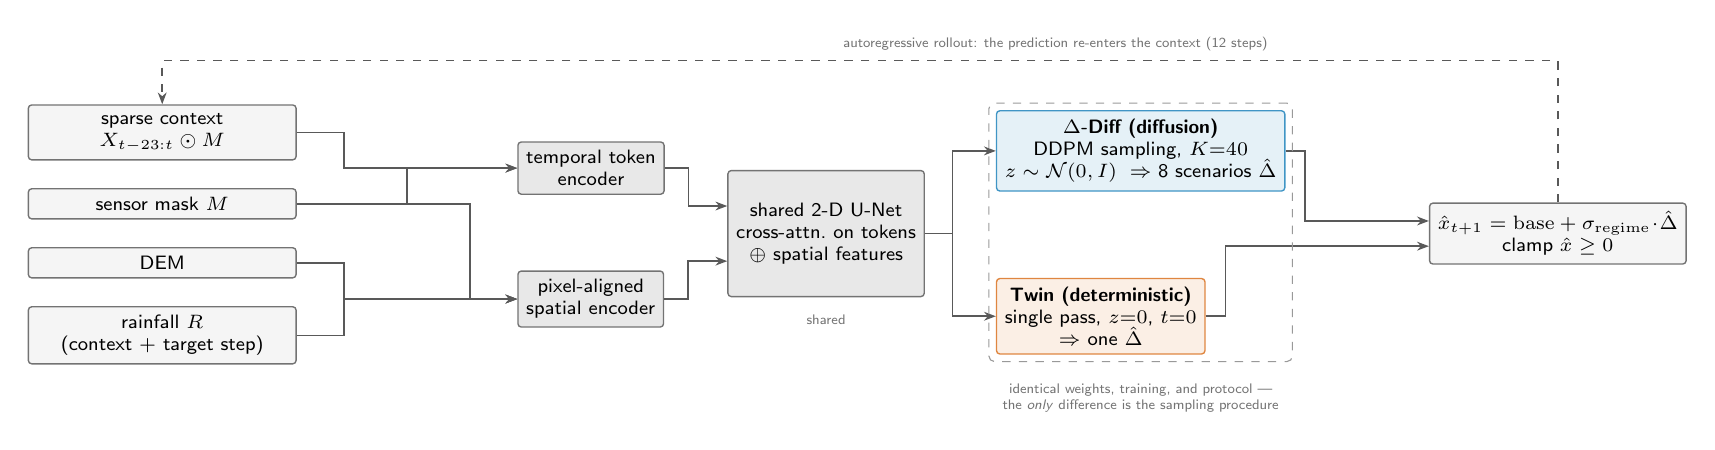
\begin{tikzpicture}[
  font=\sffamily\scriptsize,
  node distance=3.5mm and 6mm,
  box/.style={draw=black!55, rounded corners=1.2pt, align=center, inner sep=3pt, fill=black!4, line width=0.5pt},
  enc/.style={box, fill=black!9},
  headv/.style={box, fill=diffblue!10, draw=diffblue!75},
  headt/.style={box, fill=twinverm!10, draw=twinverm!75},
  arr/.style={-{Stealth[length=1.5mm]}, black!65, line width=0.55pt},
  lab/.style={font=\sffamily\tiny, black!55, align=center},
]
\node[box, minimum width=34mm] (xin) {sparse context\\ $X_{t-23:t}\odot M$};
\node[box, minimum width=34mm, below=of xin] (min) {sensor mask $M$};
\node[box, minimum width=34mm, below=of min] (dem) {DEM};
\node[box, minimum width=34mm, below=of dem] (rain) {rainfall $R$\\ (context $+$ target step)};
\coordinate (encx) at ($(rain.east)+(28mm,0)$);
\coordinate (tency) at ($(xin.east)!0.5!(min.east)$);
\coordinate (sency) at ($(dem.east)!0.5!(rain.east)$);
\node[enc, anchor=west] (tenc) at (encx |- tency) {temporal token\\ encoder};
\node[enc, anchor=west] (senc) at (encx |- sency) {pixel-aligned\\ spatial encoder};
\coordinate (unety) at ($(tenc.east)!0.5!(senc.east)$);
\coordinate (unetx) at ($(senc.east)+(8mm,0)$);
\node[enc, anchor=west, minimum height=16mm] (unet) at (unetx |- unety) {shared 2-D U-Net\\ cross-attn.\ on tokens\\ $\oplus$ spatial features};
\node[headv, anchor=west] (v2) at ($(unet.east)+(9mm,10.5mm)$) {\textbf{\ours{} (diffusion)}\\ DDPM sampling, $K{=}40$\\ $z\sim\mathcal N(0,I)\;\Rightarrow\;$8 scenarios $\hat\Delta$};
\node[headt, anchor=west] (tw) at ($(unet.east)+(9mm,-10.5mm)$) {\textbf{\twin{} (deterministic)}\\ single pass, $z{=}0$, $t{=}0$\\ $\Rightarrow$ one $\hat\Delta$};
\node[box, anchor=west] (rec) at ($(unet.east)+(64mm,0)$) {$\hat x_{t+1}=\mathrm{base}+\sigma_{\mathrm{regime}}\!\cdot\!\hat\Delta$\\ clamp $\hat x\ge 0$};
\draw[arr] (xin.east) -- ++(6mm,0) |- (tenc.west);
\draw[arr] (dem.east) -- ++(6mm,0) |- (senc.west);
\draw[arr] (rain.east) -- ++(6mm,0) |- (senc.west);
\draw[arr] (min.east) -- ++(14mm,0) |- (tenc.west);
\draw[arr] (min.east) -- ++(22mm,0) |- (senc.west);
\draw[arr] (tenc.east) -- ++(3mm,0) |- ($(unet.west)+(0,3.5mm)$);
\draw[arr] (senc.east) -- ++(3mm,0) |- ($(unet.west)+(0,-3.5mm)$);
\draw[arr] (unet.east) -- ++(3.5mm,0) |- (v2.west);
\draw[arr] (unet.east) -- ++(3.5mm,0) |- (tw.west);
\draw[arr] (v2.east) -- ++(2.5mm,0) |- ($(rec.west)+(0,1.6mm)$);
\draw[arr] (tw.east) -- ++(2.5mm,0) |- ($(rec.west)+(0,-1.6mm)$);
\draw[arr, dashed] (rec.north) -- ++(0,18mm) -| node[pos=0.18, above, lab] {autoregressive rollout: the prediction re-enters the context (12 steps)} (xin.north);
\node[draw=black!40, dashed, rounded corners=2pt, fit=(v2)(tw), inner sep=2.5pt] (differ) {};
\node[lab, below=1.5mm of differ.south] {identical weights, training, and protocol ---\\ the \emph{only} difference is the sampling procedure};
\node[lab, below=1mm of unet.south] {shared};
\end{tikzpicture}%
}
\caption{The controlled pair. Every component is shared --- inputs,
encoders, U-Net, delta-space target with per-regime scale
$\sigma_{\mathrm{regime}}$ (\S\ref{sec:regime}), training, rollout.
\ours{} draws 40 denoising steps $\times$ 8 scenarios; \twin{} evaluates
the same network once with noise and diffusion time fixed to zero. Any
performance difference is attributable to the generative mechanism.}
\label{fig:pair}
\end{figure}

\paragraph{A statistical trap in comparing the two.}
For any predictive distribution,
\begin{equation}
\mathbb{E}\big[(x_{\text{sample}} - x_{\text{truth}})^2\big]
  = \mathrm{Var}(\text{posterior}) + \mathbb{E}\big[(\bar{x} - x_{\text{truth}})^2\big]
  \;\geq\; \mathbb{E}\big[(\bar{x} - x_{\text{truth}})^2\big],
\end{equation}
so a single draw from a generative model carries strictly more expected
squared error than the predictive mean, regardless of model quality.
Comparing a single generative draw to a deterministic output on RMSE is
therefore \textbf{biased toward the deterministic model by construction}.
We encountered this bias in our own model selection during development
(Appendix~\ref{app:verification}) and corrected for it: every
decision-relevant comparison in this paper scores \ours{} by the
\emph{mean of its 8 scenarios}.

\subsection{Why the absolute field fails at fine cadence: a target-scale mechanism}
\label{sec:mechanism}
A first variant of our forecaster --- \absdiff{}, following the reference
parametrization of \citet{diffsparse2025}, diffusing the \emph{absolute}
water-depth field --- fails catastrophically at the benchmark's native
300-second cadence: in the dense regime it is $\sim$560$\times$ worse
than trivial persistence. The failure is not an implementation defect,
and the delta-space model built on the same skeleton works
(\S\ref{sec:paramresults}). What distinguishes the two is the
\emph{scale of the target}: writing $\sigma_\Delta$ for the standard
deviation of per-step changes and $\sigma_{\text{field}}$ for that of
wet-pixel depths, we measure directly from the raw data of two events
\begin{equation}
\sigma_{\text{field}} / \sigma_\Delta \;\approx\; 488 \text{ (Australia)}, \qquad 425 \text{ (UK)}
\end{equation}
(Figure~\ref{fig:mechanism}): the true per-step signal is more than two
orders of magnitude smaller than the field a model in absolute space must
reproduce. Concretely: if a model's residual error scales with the
amplitude of whatever target it is fit to, at some model-specific
constant $c$, beating persistence requires $c < \sigma_\Delta /
\sigma_{\text{field}} \approx 1/450$ in absolute space, against the far
looser $c < 1$ in delta space --- the representation choice alone moves
the bar by more than two orders of magnitude, before any modeling
decision is made.

\paragraph{Dose--response test.} Subsampling the existing frames to
larger effective time steps mechanically lowers this ratio
(Figure~\ref{fig:doseresponse}), so if target scale drives the failure,
the absolute-to-delta error ratio must fall monotonically as $\Delta t$
grows. We train one fixed skeleton under a single crossed factor
\{$\Delta t \in$ 300--7200\,s, 8 values\} $\times$ \{target: absolute,
delta\} --- one-step prediction, dense regime, seed 42, screening
protocol. The pre-registered criterion (monotone decrease) is met at
every step (Table~\ref{tab:doseresponse}), and the ratio follows the
predicted power law closely: log--log slope $-1.06$ ($R^2=0.98$),
matching the $-1$ exponent implied by the near-linear growth of
$\sigma_\Delta$ with $\Delta t$.

\begin{table}[H]
\centering
\caption{Dose--response (one-step, dense, seed 42): RMSE of the
absolute- and delta-target arms at each $\Delta t$, and their ratio.
Monotone decrease 8/8 --- the pre-registered criterion.}
\label{tab:doseresponse}
\begin{tabular}{rrrr}
\toprule
$\Delta t$ (s) & \absdiff{} RMSE (m) & \ours{} RMSE (m) & Ratio \\
\midrule
300  & 0.3788 & 0.000175 & 2162 \\
600  & 0.3676 & 0.000326 & 1127 \\
900  & 0.3729 & 0.000471 & 792 \\
1200 & 0.3717 & 0.000606 & 614 \\
1800 & 0.3729 & 0.000899 & 415 \\
2400 & 0.3821 & 0.001250 & 306 \\
4800 & 0.3962 & 0.002530 & 157 \\
7200 & 0.3965 & 0.006507 & 61 \\
\bottomrule
\end{tabular}
\end{table}

\paragraph{The effect is not diffusion-specific.} Two observations
suggested the law might not be about generative sampling at all: the
absolute arm's error is nearly constant across the entire $\Delta t$
range (0.368--0.397\,m), and the delta arm's error closely tracks the
independently measured $\sigma_\Delta(\Delta t)$
(Appendix~\ref{app:doseresponse}). We therefore ran the decisive control:
the identical 16-run design on \twin{}, with no diffusion sampling
anywhere. The twin reproduces the same power law --- slope $-0.916$,
$R^2=0.987$, all 8 of 8 $\Delta t$ points, closely matching the diffusion
arm's $-1.06$/$0.98$. The
conclusion is sharper than the hypothesis we set out to test: what is
demonstrated is a \textbf{target-scale mechanism} --- regression error
tracks the scale of the chosen target, so a fine-cadence absolute-field
target buries the physical signal for \emph{any} model of this family,
generative or not. This strengthens the paper's central attribution
thesis: even the reference parametrization's failure, the strongest
apparent evidence for diffusion-specific reasoning in this line of work,
is representation-driven. A secondary finding: the delta target itself
stops beating persistence beyond $\Delta t\approx 65$\,min (interpolated
crossing $\approx$3910\,s), where genuine change accumulates enough that
``predict no change'' is no longer weak
(Appendix~\ref{app:doseresponse}).

\begin{figure}[H]
  \centering
  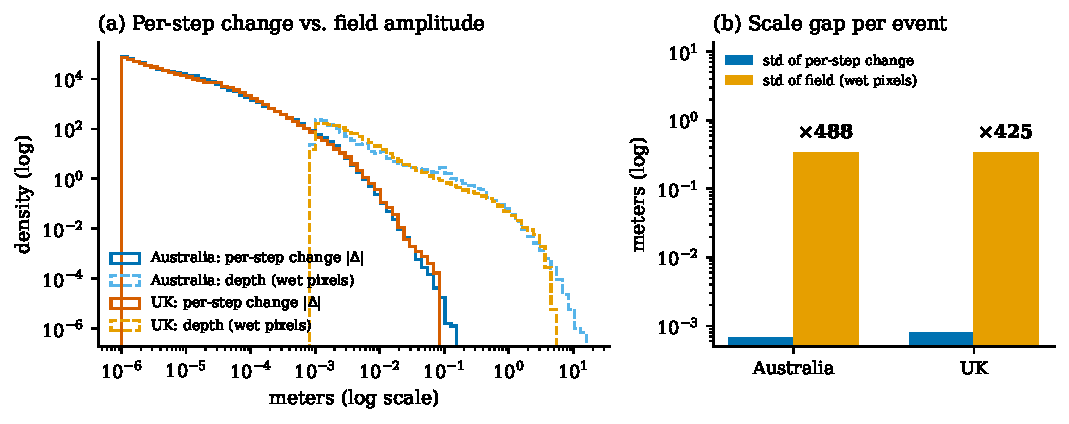
\includegraphics[width=0.92\linewidth]{figures/f2_mechanism.pdf}
  \caption{Target-scale mismatch measured from raw data of two events:
  per-step changes $|\Delta|$ sit two to three orders of magnitude below
  wet-pixel depths, a $\sim$488$\times$ (Australia) / $\sim$425$\times$
  (UK) gap.}
  \label{fig:mechanism}
\end{figure}

\begin{figure}[H]
  \centering
  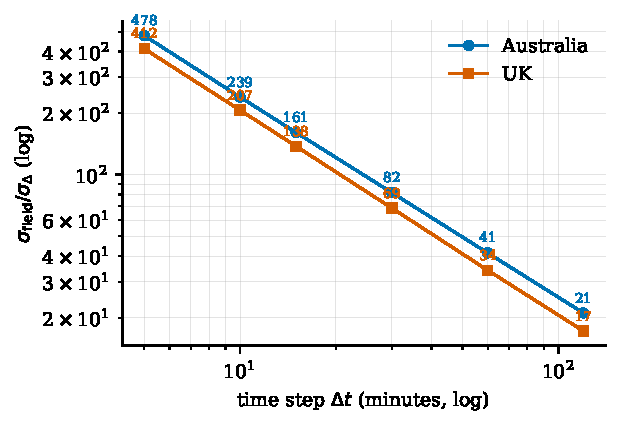
\includegraphics[width=0.7\linewidth]{figures/f2b_dose_response_ratio.pdf}
  \caption{Measured $\sigma_{\text{field}}/\sigma_\Delta$ vs.\ effective
  $\Delta t$ (frame subsampling, data only): $\sigma_\Delta$ grows
  near-linearly, so the ratio falls as $\sim 1/\Delta t$ (478$\to$21
  Australia, 412$\to$17 UK). The marked $\Delta t$ values are the
  training points of Table~\ref{tab:doseresponse}.}
  \label{fig:doseresponse}
\end{figure}

\subsection{Per-regime scale under partial observation}
\label{sec:regime}
Under sparsity, at an observed pixel the natural target scale is the
change from its last known value ($\sigma_\Delta$); at a masked pixel the
target is the change from a training-mean fill, whose scale is closer to
$\sigma_{\text{field}}$. A single global normalization either drowns the
observed-pixel signal or destabilizes the masked-pixel one --- an
instability we hit directly during development
(Appendix~\ref{app:verification}). \ours{} therefore uses a
\textbf{per-pixel, regime-aware scale} $\sigma_{\mathrm{regime}}$,
resolved at each pixel from its observed/masked status.

\subsection{Architecture summary}
\absdiff{} uses the reference architecture of \citet{diffsparse2025} with
a 12-frame context. \ours{} widens the temporal token encoder, adds a
pixel-aligned spatial conditioning pathway, and extends the context to 24
frames. Because the longer context is a potential confounder, we ablate
it: \ours{} retrained at the \emph{same} 12-frame context retains
essentially the entire advantage (dense $970\times$, \mfifty{}
$3.9\times$, \mninetyfive{} $1.9\times$ over \absdiff{}, screening
evaluation). \blocked{The context ablation is single-seed; two further
seeds are planned before freeze.}

% ============================================================
\section{Evaluation Protocol}
\label{sec:protocol}

All headline numbers use the benchmark's full test protocol: the test
split of each event (Table~\ref{tab:datasets}; 13 evaluation windows of
24 context $+$ 12 prediction frames for Australia), tiled rollout over
overlapping $64\times64$ patches (stride 32) with Hann-blended seams,
and, for \ours{}, 8 sampled scenarios scored by their mean
(\S\ref{sec:twin}). Evaluation masks come from a fixed seeded bank shared
across all models and seeds. Two persistence references anchor every
table: \emph{oracle} persistence (no change, from the true dense field)
and \emph{sparse} persistence (no change, from the masked observation).
Every headline comparison reports mean $\pm$ std over 3 training seeds;
no single-seed number appears without a screening label.

\paragraph{Convergence audit.} Midway through the study, an audit found
sparse-regime checkpoints of \emph{both} models under-trained; every
sparse-regime number here comes from checkpoints retrained under an
extended budget, and the central verdict was re-derived from scratch ---
with no change in conclusion (Appendix~\ref{app:verification}).

\paragraph{Significance.} The main check is a seed-paired sign test:
whether the per-seed difference (\ours{} $-$ \twin{}) keeps one sign
across all 3 seeds. The evaluator also logs per-window metrics, enabling
a window$\times$seed paired test; evaluation windows overlap (stride 20,
window 36), so they are not independent samples, and we treat
window-level tests as supporting rather than primary evidence.

% ============================================================
\section{Results}
\label{sec:results}

\subsection{A new state of the art under full observation}
\label{sec:vsfnoplus}
Our own FNO+ reproduction sits $1.66\times$ above the published relative
RMSE --- a gap we attribute to undisclosed preprocessing after
eliminating implementation error --- so we compare against the
\emph{published} FNO+ numbers directly \citep{floodcastbench2025},
sidestepping the reproduction question. \ours{} outperforms on all five
reported metrics (Table~\ref{tab:vsfnoplus}).

\begin{table}[H]
\centering
\caption{\ours{} under full observation (mean $\pm$ std, 3 seeds, full
test protocol) vs.\ \emph{published} FNO+ on the same split.
\textbf{Bold} marks the better value.}
\label{tab:vsfnoplus}
\begin{tabular}{lrr}
\toprule
Metric & FNO+ (published) & \ours{} (ours) \\
\midrule
Relative RMSE $\downarrow$ & 0.003941 & $\mathbf{0.001558 \pm 0.000836}$ \\
NSE $\uparrow$              & 0.999979 & $\mathbf{0.999996 \pm 0.000004}$ \\
Pearson $r$ $\uparrow$      & 0.999990 & $\mathbf{0.999999 \pm 0.000001}$ \\
CSI@0.001\,m $\uparrow$     & 0.939638 & $\mathbf{0.985861 \pm 0.003884}$ \\
CSI@0.01\,m $\uparrow$      & 0.984588 & $\mathbf{0.999063 \pm 0.000416}$ \\
\bottomrule
\end{tabular}
\end{table}

\paragraph{The stronger result is the twin.} \twin{} reaches a dense
relative RMSE of $0.000417 \pm 0.000039$
(Table~\ref{tab:twinresults}): $\sim$\textbf{9.4$\times$ below the
published state of the art}, from a single forward pass where \ours{}
spends 40 denoising steps $\times$ 8 scenarios. The same holds on the
benchmark's low-fidelity task: trained on Pakistan (480\,m), \twin{}
reaches relative RMSE $0.000317 \pm 0.000172$ vs.\ published FNO+
0.002107 ($\sim$6.6$\times$, ahead on all five metrics with 3 seeds;
per-seed values and a convergence caveat on one seed in
Appendix~\ref{app:perseed}). Protocol differences are stated once:
published FNO+ numbers are single-shot 19-step predictions, ours are
autoregressive 12-step rollouts (compounding errors, but a shorter
horizon); \ours{} is scored by its 8-scenario mean while \twin{}, like
FNO+, is a single deterministic output. Input context does not explain
the margin either: retraining FNO+ \emph{with} our 24-frame context makes
it worse, not better ($0.007529\pm0.000328$ vs.\ its own
$0.006550\pm0.000135$, 3 seeds).

\subsection{Parametrization dominates; context length does not explain it}
\label{sec:paramresults}
Figure~\ref{fig:sparsity} compares the model family across observation
regimes. The delta-space parametrization is worth up to three orders of
magnitude: \absdiff{} sits at or above persistence everywhere, while
every delta-space model is far below it --- as the target-scale mechanism
of \S\ref{sec:mechanism} predicts. The short-context ablation confirms
the advantage is not input history (\S\ref{sec:vsfnoplus} showed the same
for the baseline).

\begin{figure}[H]
  \centering
  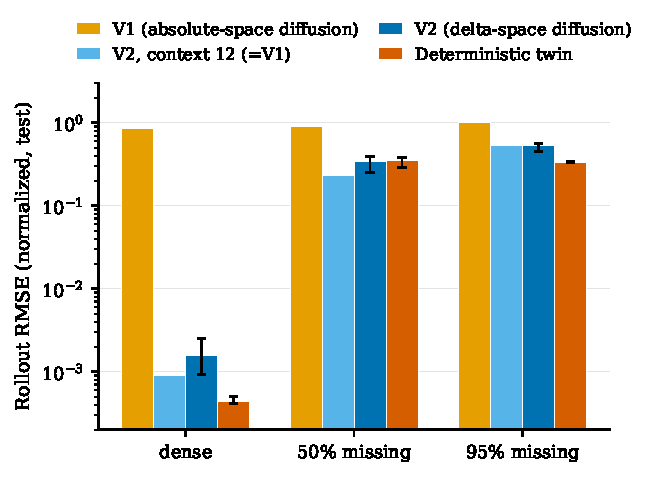
\includegraphics[width=0.78\linewidth]{figures/f3_performance_sparsity.pdf}
  \caption{Rollout RMSE (normalized, test set, log scale) across
  observation regimes. \absdiff{} and short-context \ours{}: single-seed
  screening; \ours{} and \twin{}: mean of 3 seeds, error bars span the
  seed range.}
  \label{fig:sparsity}
\end{figure}

\subsection{Diffusion vs.\ its twin on the primary event}
\label{sec:twinresults}

\begin{figure}[H]
  \centering
  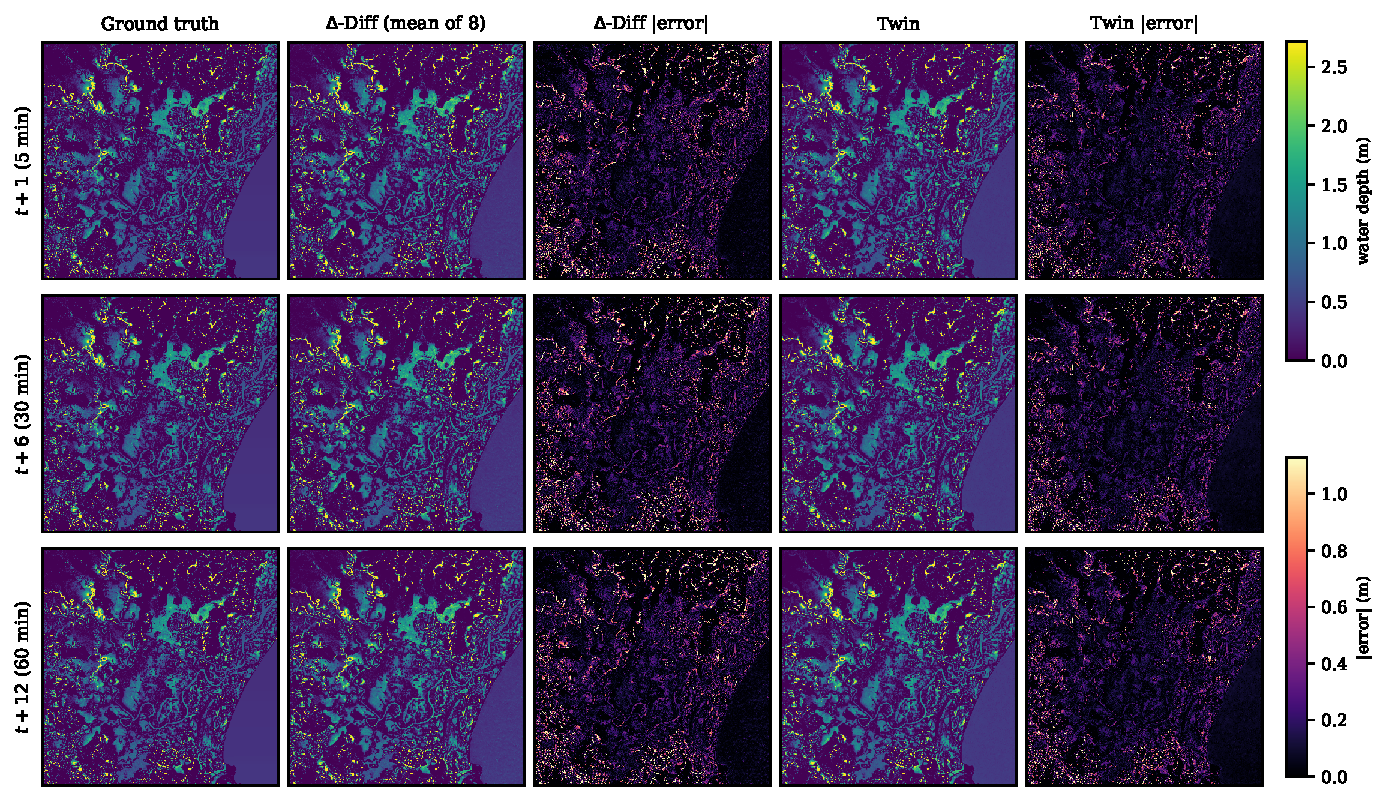
\includegraphics[width=0.72\linewidth]{figures/f7_qualitative_maps.pdf}
  \caption{Qualitative rollout at \mninetyfive{}, one representative test
  window; colormaps capped at the 99th percentile. \twin{}'s error map is
  visibly darker (mean absolute error $\approx$0.105\,m vs.\
  $\approx$0.122\,m for \ours{}); errors concentrate at flood boundaries
  for both.}
  \label{fig:qualitative}
\end{figure}

The decision criteria were pre-registered: a \twin{} sweep would mean the
generative mechanism adds nothing here; \ours{} winning under sparsity
would confirm the generative premise; any mixed outcome is reported
per-regime with no blanket claim. The outcome is \textbf{mixed}
(Table~\ref{tab:twinresults}): \twin{} dominates at both extremes ---
dense, where there is no reconstruction ambiguity to resolve, and
\mninetyfive{}, where a naive prior would expect the generative advantage
to be \emph{largest} --- while \mfifty{} is genuinely undecided, the sign
flipping between seeds. This non-monotone pattern is more informative
than a clean sweep: sparsity level alone does not predict a generative
advantage, and a tautology would predict uniform dominance. The verdict
is robust: it is unchanged from a pre-correction read on the original
checkpoints ($\times$3.55/quasi-tie/$\times$1.57), and at \mninetyfive{}
\twin{} leads on all six metrics we compute while at \mfifty{} \emph{no}
metric shows a seed-consistent direction.

\begin{table}[H]
\centering
\caption{\ours{} (mean of 8 scenarios) vs.\ \twin{}, relative RMSE, mean
$\pm$ std over 3 seeds, full test protocol, Australia. Rightmost column:
does the per-seed difference keep one sign across all 3 seeds?}
\label{tab:twinresults}
\begin{tabular}{lrrll}
\toprule
Regime & \ours{} & \twin{} & Winner & Consistent sign \\
\midrule
dense & 0.001558 $\pm$ 0.000836 & $\mathbf{0.000417 \pm 0.000039}$ & \twin{}, $\times$3.7 & yes \\
\mfifty{} & $\mathbf{0.318425 \pm 0.043702}$ & 0.348852 $\pm$ 0.040779 & \ours{}, $\times$1.1 (weak) & \textbf{no} \\
\mninetyfive{} & 0.492443 $\pm$ 0.013940 & $\mathbf{0.344249 \pm 0.006248}$ & \twin{}, $\times$1.4 & yes \\
\bottomrule
\end{tabular}
\end{table}
\FloatBarrier

\subsection{Second event, in-domain: the pattern simplifies}
\label{sec:ukresults}
We replicate the full protocol --- both models, 3 seeds, all three
sparsity regimes, 18 training runs --- on the UK event, trained from
scratch in-domain (Table~\ref{tab:ukresults}). Here the twin wins
\emph{all three} regimes with a consistent sign across all 3 seeds in
each, including the intermediate regime that was undecided on Australia.
Margins are tighter ($\times$1.06--1.14 vs.\ Australia's
$\times$1.4--3.7), consistent with the much smaller domain. Across the
two events the summary is: \textbf{the generative mechanism never shows a
seed-consistent advantage in any regime on either event}, while the twin
shows one in five of six event$\times$regime cells. Per-seed values in
Appendix~\ref{app:perseed}.

\begin{table}[H]
\centering
\caption{UK event, in-domain (mean $\pm$ std, 3 seeds, full test
protocol), relative RMSE.}
\label{tab:ukresults}
\begin{tabular}{lrrll}
\toprule
Regime & \ours{} & \twin{} & Winner & Consistent sign \\
\midrule
dense & 0.006018 $\pm$ 0.000590 & $\mathbf{0.005674 \pm 0.000416}$ & \twin{}, $\times$1.06 & yes \\
\mfifty{} & 0.174123 $\pm$ 0.011544 & $\mathbf{0.156572 \pm 0.004881}$ & \twin{}, $\times$1.11 & yes \\
\mninetyfive{} & 0.223112 $\pm$ 0.008981 & $\mathbf{0.194904 \pm 0.008246}$ & \twin{}, $\times$1.14 & yes \\
\bottomrule
\end{tabular}
\end{table}

\subsection{Cross-regional transfer, zero-shot}
\label{sec:zeroshot}
FloodCastBench's authors also evaluate FNO+ zero-shot: weights trained on
one event, frozen, evaluated on another. We replicate this protocol
(frozen weights \emph{and} frozen normalization) on both published
transfer pairs, evaluating on each target event's \emph{full} frame
sequence --- legitimate in zero-shot, since no target frame was ever
trained on, and necessary: our first pass on the usual small held-out
splits produced ratios inflated $\sim$4--10$\times$ by
unrepresentatively calm slices (Appendix~\ref{app:transferpitfall}).

\begin{table}[H]
\centering
\caption{Zero-shot transfer, relative RMSE vs.\ published FNO+ under the
same frozen-weights protocol, on each target event's full frame
sequence. \twin{} is a single deterministic output, matching FNO+'s
output type.}
\label{tab:zeroshot}
\begin{tabular}{llrr}
\toprule
Transfer pair & Model & relRMSE $\downarrow$ & vs.\ FNO+ \\
\midrule
Australia$\to$UK (42 windows) & FNO+ \citep{floodcastbench2025} & 0.024771 & --- \\
 & \twin{} (3 seeds) & $\mathbf{0.002874 \pm 0.000177}$ & $\sim$\textbf{8.6$\times$} \\
\midrule
Pakistan$\to$Mozambique (85 windows) & FNO+ \citep{floodcastbench2025} & 0.078633 & --- \\
 & \twin{} (3 seeds) & $\mathbf{0.006249 \pm 0.003625}$ & $\sim$\textbf{12.6$\times$} \\
\bottomrule
\end{tabular}
\end{table}

Both pairs point the same direction. The margin decomposes informatively:
on Mozambique the twin beats trivial persistence by only
$\sim$8$\times$ --- most of the $\sim$12.6$\times$ comes from FNO+
transferring far \emph{worse} than persistence. This is the target-scale
mechanism again: an absolute-field model must reproduce the target
domain's absolute depth distribution, which shifts across regions, while
a delta-parametrized model needs only the per-step change distribution,
which barely does. The Pakistan$\to$Mozambique spread is dominated by one
seed with a training-convergence failure (Appendix~\ref{app:perseed});
the two healthy seeds sit at 0.00363--0.00375 ($\sim$21$\times$). \ours{}
evaluated on the same full-event protocol is consistently behind the twin
(Appendix~\ref{app:transferpitfall}). Remaining caveat: the publication
does not specify whether its transfer numbers froze source-domain
normalization as ours do.

\subsection{Structured sensor layouts vs.\ random masks}
\label{sec:masks}
Training uses i.i.d.\ random masks; real sensor networks are not i.i.d.
We evaluate two structured mask families never seen in training, at
matched sensor budget (Table~\ref{tab:masks}). The \textbf{gauge} mask
--- structured but spatially distributed --- transfers almost perfectly.
The \textbf{cluster} mask leaves a large contiguous region unobserved, a
spatial regime never encountered in training, and degrades markedly: the
model's implicit assumption is \emph{distributed} partial observation,
not merely a sensor count --- a deployment limitation worth stating
plainly.

\begin{table}[H]
\centering
\caption{\ours{} relative RMSE under structured vs.\ random masks at
matched sensor budget (seed 42; cluster/\mfifty{} confirmed on a second
seed: 0.597 vs.\ 0.609).}
\label{tab:masks}
\begin{tabular}{lrrl}
\toprule
Mask & \mfifty & \mninetyfive & vs.\ random \\
\midrule
Random (training distribution) & 0.395 & 0.567 & --- \\
Gauge (spatially distributed)  & 0.393 & 0.585 & $\approx$ identical \\
Cluster (contiguous gap)       & 0.609 & 0.706 & \textbf{+54\% / +25\%} \\
\bottomrule
\end{tabular}
\end{table}

\subsection{Calibration}
\label{sec:calibration}
\ours{}'s 8-scenario ensembles show \textbf{severe, systematic
under-coverage} in every tested condition
(Figure~\ref{fig:calibration}): a nominal 90\% interval
(finite-ensemble corrected) covers only 20--47\% of true outcomes.
Sparsity level, not mask structure, dominates calibration quality ---
counter-intuitively, \mninetyfive{} is better calibrated than \mfifty{}.

\begin{figure}[H]
  \centering
  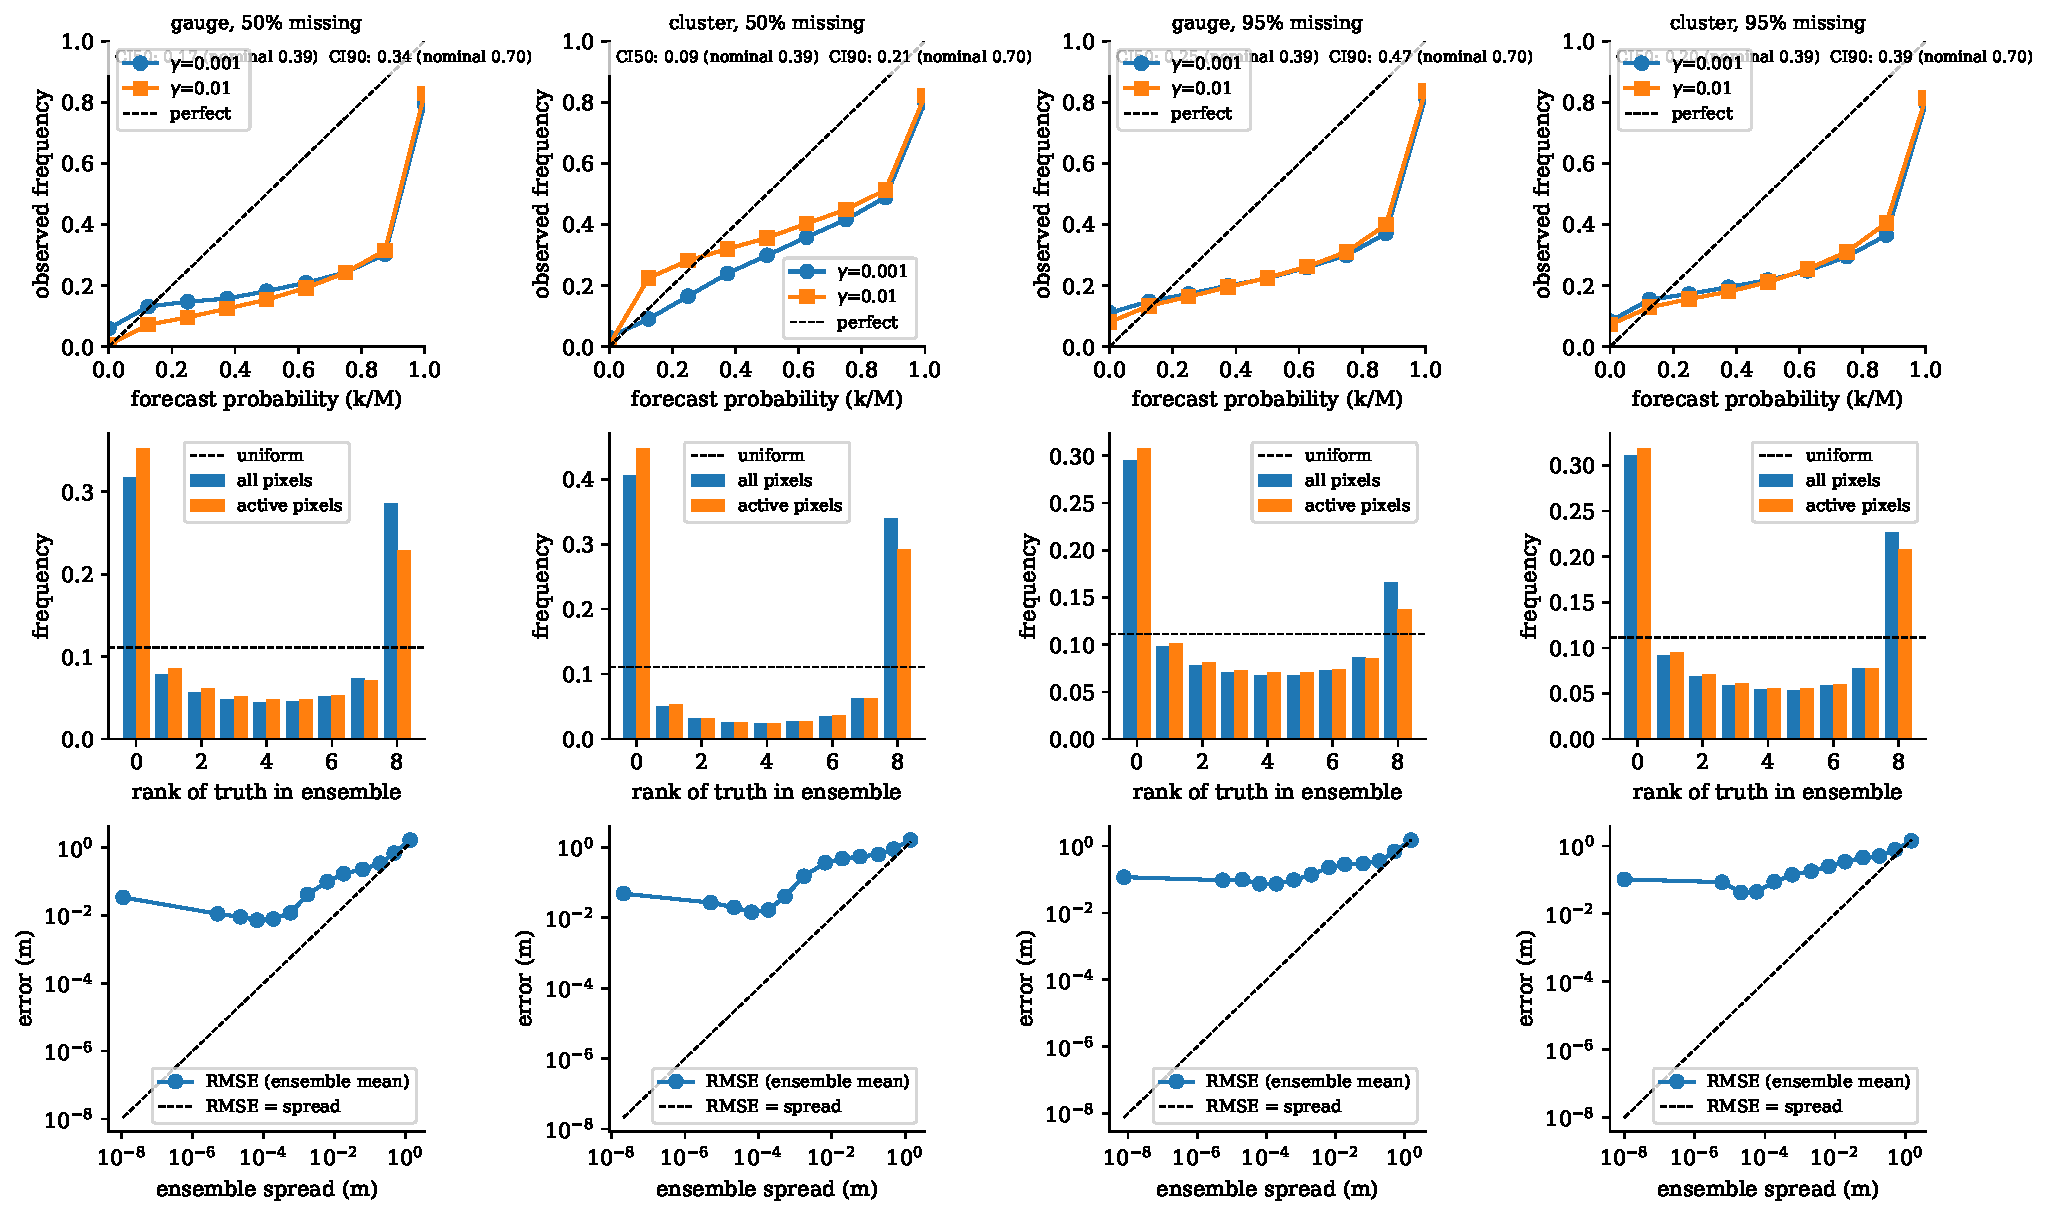
\includegraphics[width=0.9\linewidth]{figures/f5_calibration_diagnostics.pdf}
  \caption{Calibration diagnostics for \ours{} across mask $\times$
  sparsity conditions: wet/dry reliability, rank histograms, spread vs.\
  error. Under-coverage is systematic everywhere.}
  \label{fig:calibration}
\end{figure}

\paragraph{Is a generative model even needed for uncertainty?}
The rejoinder ``a deterministic model cannot quantify uncertainty'' is
false as stated: a \emph{deep ensemble} of independently trained
deterministic models \citep{lakshminarayanan2017deep} is the standard
baseline, and our three \twin{} seeds provide one at zero additional
cost. At \mfifty{} the twin ensemble ($M{=}3$) covers 47\% of its
corrected 50\%-interval nominal vs.\ \ours{}'s 40\% ($M{=}8$, matched
random masks); at \mninetyfive{}, 70\% vs.\ 64\% (gauge) / 52\%
(cluster). \textbf{At no sparsity tested is the twin ensemble less well
calibrated than the diffusion ensemble} (Figure~\ref{fig:calibcomp}), and
the rank histograms show the diffusion ensemble as, if anything, more
overconfident. The uncertainty-based defense of diffusion is not merely
unproven here --- it is contradicted by the one baseline it should be
compared against.

\begin{figure}[H]
  \centering
  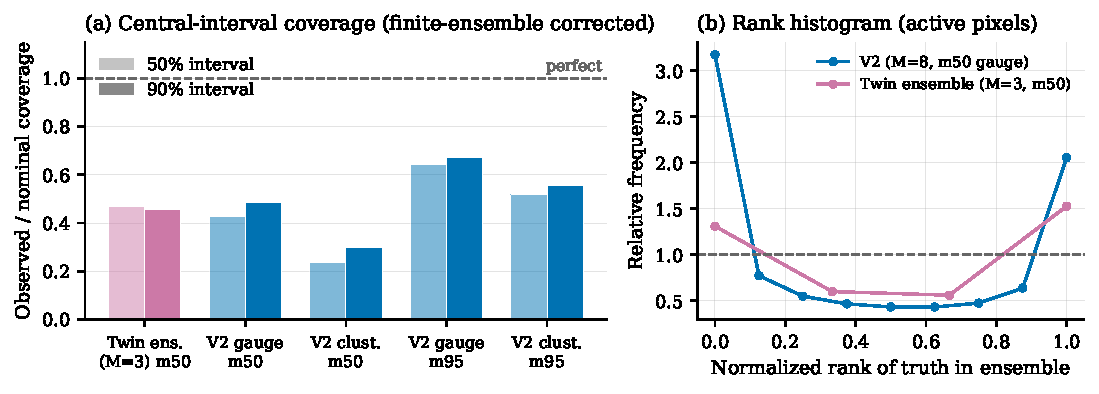
\includegraphics[width=\linewidth]{figures/f6_calibration_comparison.pdf}
  \caption{Diffusion ensembles vs.\ a deep ensemble of twins:
  (a) observed/nominal coverage --- all conditions under-covered, twin
  ensemble never worse; (b) rank histograms at \mfifty{} --- both
  U-shaped, \ours{} more strongly. At \mninetyfive{} \ours{} uses
  structured masks, which \S\ref{sec:masks} suggests understates rather
  than overstates its calibration; a matched random-mask evaluation at
  \mninetyfive{} (relRMSE 0.508, statistically indistinguishable from the
  regime mean) confirms the reading is not mask-structure-driven.}
  \label{fig:calibcomp}
\end{figure}

\paragraph{Sharpness.} Coverage alone cannot distinguish a well-calibrated
ensemble from one that is merely wide; a sharpness-aware score answers the
question completely. \ours{}'s normalized CRPS averages
$0.1599\pm0.0257$ at \mfifty{} and $0.3488\pm0.0077$ at \mninetyfive{}
(3 seeds, random masks, dense-regime scale of the same metric is two
orders of magnitude smaller and not directly comparable across regimes).
Combined with the under-coverage above, the picture is internally
consistent: the ensemble is simultaneously too narrow (fails coverage)
and not particularly cheap in spread (nonzero CRPS) --- it is not merely
conservative-but-wide, it is misplaced.

\blocked{Remaining: integrating the random-mask \mninetyfive{}
evaluation's finite-ensemble-corrected coverage into
Figure~\ref{fig:calibcomp} (raw evaluation complete, twice ---
independently reproduced to 4 decimal places), and a sharpness-aware
score (CRPS) to complement coverage.}

\subsection{Ablations and cost}
\label{sec:ablations}

\paragraph{Measured cost.} Table~\ref{tab:cost} prices the diffusion loop
directly: both models load their trained checkpoints and predict one real
$64\times64$ tile on the same GPU (\ours{}: 40 denoising steps $\times$ 8
scenarios, batched; \twin{}: one forward pass). The parameter match is
exact by construction and verified at load time. The wall-clock gap
($\sim$58$\times$) is smaller than the 320$\times$ network-evaluation
count because batching amortizes per-call overhead --- we report both
rather than let the larger number stand alone.

\begin{table}[H]
\centering
\caption{Measured inference cost, one $64\times64$ tile prediction,
mean of 5 repetitions on the same device.}
\label{tab:cost}
\begin{tabular}{lrr}
\toprule
 & \ours{} & \twin{} \\
\midrule
Parameters & 5{,}538{,}546 & 5{,}538{,}546 \\
Network evaluations / prediction & 320 & 1 \\
Latency (s) & 0.792 & $\mathbf{0.0137}$ \\
Peak GPU memory (MB) & 152 & $\mathbf{92}$ \\
\bottomrule
\end{tabular}
\end{table}

\paragraph{Component ablation, first lever: delta parametrization alone.}
Holding \ours{}'s architecture fixed and swapping only the target back to
\emph{absolute} (single-seed screening, dense, 4 test windows) gives
relative RMSE $0.309516$ --- $\mathbf{\sim199\times}$ worse than \ours{}
($0.001558$ on the full protocol). This isolates the delta
parametrization's own contribution from the architectural changes
(\S\ref{sec:mechanism}, \S\ref{sec:paramresults}): it dominates the
$\sim$3-order-of-magnitude gap over \absdiff{}, with the widened
architecture contributing comparatively little (this ablation's absolute
score is already far better than \absdiff{}'s reference-parametrization
result, \S\ref{sec:mechanism}, despite sharing \absdiff{}'s absolute
target).

\paragraph{Second lever: change-weighted loss.} Removing the wet/dry
boundary loss weighting (single-seed screening, dense, 4 windows) gives
relative RMSE $0.001811$ --- only $\sim$1.16$\times$ worse than \ours{}
($0.001558\pm0.000836$), within one seed standard deviation, and its
CSI@0.001 ($0.984760$) is statistically indistinguishable from \ours{}'s
($0.985861\pm0.003884$). Unlike the delta parametrization, this lever's
effect is not detectable at screening resolution --- consistent with its
design intent (a boundary-sharpening reweighting) mattering more for
sharper, harder-to-measure boundary metrics than for pooled RMSE/CSI.

\paragraph{Third lever: rollout-aware (pushforward) training.} Removing
the exposure-bias curriculum (single-seed screening, dense, 4 windows)
gives relative RMSE $0.000865$ --- numerically \emph{better} than
\ours{} ($0.001558\pm0.000836$), not worse. We do not read this as
evidence that pushforward training hurts: \ours{}'s own dense-regime
seed standard deviation is more than half its mean, so a single
screening seed landing below the 3-seed mean is well within the noise
this technique already shows at full protocol (\S\ref{sec:vsfnoplus}).
Unlike the delta parametrization (a $\sim$199$\times$ effect, far
outside any plausible noise band), this lever's direction cannot be
called from one seed; it is reported as inconclusive pending the
3-seed confirmation already planned for the full ablation grid.

\paragraph{Fourth lever: pixel-aligned spatial encoder.} Removing the
spatial conditioning pathway (DEM, rainfall, sensor mask; single-seed
screening, dense, 4 windows) gives relative RMSE $0.001903$
($\sim$1.22$\times$ \ours{}, still inside the noise band above) but
CSI@0.001 drops to $0.900702$ --- $\sim$22 seed-standard-deviations
below \ours{}'s $0.985861\pm0.003884$, far outside any plausible noise
reading. The dissociation is informative: removing spatial context
barely moves aggregate error but substantially degrades wet/dry
boundary detection specifically, consistent with the pathway's role
(terrain and forcing are boundary-relevant, not magnitude-relevant).

\blocked{Remaining: two further levers of the component ablation
(target-step rainfall, diffusion steps) --- training in progress, 4 of
6 configurations complete. 3-seed confirmations warranted for the
pushforward lever (single-seed result outside the pattern of the
others) and optionally the spatial-encoder CSI drop.}

% ============================================================
\section{Discussion}
\label{sec:discussion}

\paragraph{When does generative forecasting pay off here?} Nowhere with
consistent sign, and the fine structure is informative. On Australia,
\twin{} wins decisively at both ends of the observability spectrum ---
dense, where there is no reconstruction ambiguity to resolve, and
\mninetyfive{}, where the field's calibration intuition would put the
generative advantage at its \emph{largest} --- with \mfifty{} undecided;
on UK, \twin{} sweeps all three regimes. Sparsity level does not predict
a generative advantage on this benchmark, which is sharper and less
convenient than either pre-registered blanket claim.

\paragraph{Where the gains actually come from.} The attribution question
has a measurable answer. The three-orders-of-magnitude jump from
\absdiff{} to \ours{} comes from the delta-space target and regime-aware
scale (\S\ref{sec:paramresults}); it survives removing the extra context;
it transfers \emph{in full} to the deterministic twin, which then goes
further; and the dose--response law behind the reference
parametrization's failure is reproduced by the twin itself
(\S\ref{sec:mechanism}) --- it is a property of the target, not of the
sampler. Nothing in our measurements requires the generative mechanism to
explain any gain. Whether the residual, seed-inconsistent \mfifty{}
margin on Australia reflects a real narrow niche for generative
forecasting or seed noise cannot be resolved at 3 seeds; UK's sweep
suggests the latter.

\paragraph{Epistemic vs.\ aleatoric, and what diffusion was imported
for.} Generative forecasting earned its place in domains with genuine
trajectory-level stochasticity \citep{gencast2024}. FloodCastBench's
ground truth is a single deterministic simulation: the only uncertainty
partial observation introduces is epistemic --- reconstruction ambiguity,
which shrinks with information rather than growing with lead time. Our
results are what that distinction predicts, including the calibration
outcome (\S\ref{sec:calibration}). The noise-free-vs-noisy contrast of
\citet{spatiallyawarediffusion2024} suggests the boundary shifts once
observations carry noise --- our benchmark's synthetic sensors do not, a
scope condition we state rather than hide.

\paragraph{Is the twin an FNO replacement? A scoped answer.} The twin
beats FNO+ in-domain ($\sim$9.4$\times$ and $\sim$6.6$\times$ on two
events) and on both published zero-shot transfer pairs
($\sim$8.6$\times$, $\sim$12.6$\times$). We answer deliberately narrowly.
The inductive bias that favors it here --- local multi-scale convolution
and attention, suited to sharp, localized wetting fronts under sparse
observation --- is the same bias that predicts it should \emph{lose} on
the globally smooth fields FNO was designed for, where spectral mixing
and resolution-invariance are genuine advantages \citep{li2021fno}. No
architecture dominates across problem classes; testing on FNO's home
terrain is the right future adversarial experiment. What our results
support is the scoped statement: for sparse-observation forecasting of
sharp-fronted flood fields, this design point is preferable to FNO+ on
every axis we measured. Two confounds remain even for that claim: the
twin differs from FNO+ in both backbone and parametrization, and
separating the two requires giving FNO+ the delta-space, regime-aware
target --- the decisive next experiment on this axis.

\paragraph{A procedural corollary.} Everything above was only visible
because a parameter-matched deterministic twin existed --- a
configuration change, not a new model. It converted ``our diffusion model
beats the baseline'' into ``our representation choices beat the baseline;
the sampler subtracts value.'' We suggest the practice, stated modestly:
\emph{before attributing a forecasting gain to a generative mechanism,
evaluate the same network with the mechanism switched off.} A single
demonstration that this control can reverse a paper's headline
attribution is, we think, sufficient motivation; it does not require our
substantive findings to generalize beyond this benchmark, and we claim no
such generalization (\S\ref{sec:limitations}).

\subsection{Limitations}
\label{sec:limitations}
\begin{itemize}
  \item Ground truth is one deterministic simulation per event:
    calibration claims are scoped to reconstruction ambiguity
    (\S\ref{sec:calibmeaning}).
  \item Sparsity is synthetic (random + two structured families), and
    sensors are noise-free --- the regime
    \citet{spatiallyawarediffusion2024} identify as maximally favorable
    to deterministic models; an observation-noise axis is future work.
  \item In-domain results cover two events of one benchmark (a third,
    Pakistan, at reduced protocol); zero-shot transfer covers its two
    published pairs at 3 seeds each, with one seed a documented
    convergence outlier (Appendix~\ref{app:perseed}) and one
    unverifiable protocol detail (whether published transfer numbers
    froze source normalization as ours do).
  \item Significance rests on seed-paired sign tests ($n{=}3$);
    evaluation windows overlap and are not independent, so window-level
    tests are supporting evidence only. The \mfifty{} verdict on
    Australia (sign flip at 3 seeds) cannot distinguish a genuine
    near-tie from seed noise.
  \item Even four events are draws from one simulator and one curation
    pipeline --- a pattern holding across all of them could still be a
    property of the simulator rather than of flood dynamics. We
    therefore separate the \emph{procedural} recommendation (check any
    claimed generative advantage against a matched twin), which one
    rigorous demonstration supports, from the \emph{substantive}
    finding (the specific pattern we measure), which is scoped to
    FloodCastBench and the architectures tested.
\end{itemize}

% ============================================================
\section*{Reproducibility Statement}
Code, configurations, and seeds for every reported run are version
controlled. All headline comparisons use $\geq 3$ seeds; single-seed
numbers carry explicit screening labels. Every comparison holds input
context and evaluation protocol fixed, and remaining asymmetries are
stated next to the numbers they affect. Appendix~\ref{app:verification}
catalogues the pipeline errors we caught during the project --- each
found by verification practices we now consider part of the method ---
including one (the transfer small-sample pitfall,
Appendix~\ref{app:transferpitfall}) that would otherwise have inflated a
headline claim by a factor of four to ten.
\blocked{Repository URL will be added when the draft is frozen.}

% ============================================================
\appendix

\section{Verification practices and caught pitfalls}
\label{app:verification}

Each of the following was caught by a verification step before it could
distort a conclusion; we list them because the catalogue is, in our
view, as instructive as the results.

\begin{enumerate}
  \item \textbf{Single-draw comparison bias} (\S\ref{sec:twin}). An
    internal validation metric scored \ours{} by a single rollout draw,
    mathematically favoring the deterministic model. Caught during
    development; all decision-relevant comparisons now score the
    8-scenario mean. Codified as a permanent project rule.
  \item \textbf{Convergence audit --- with one asymmetry caught by a
    second audit.} Sparse-regime checkpoints were under-trained under the
    original budget (retraining improved \ours{}'s internal selection
    metric by 16--37\%). \mninetyfive{} checkpoints of both models and
    \ours{}'s \mfifty{} checkpoints were retrained under an extended
    budget and all their numbers re-derived; the central verdict was
    unchanged ($\times$3.55/quasi-tie/$\times$1.57 before vs.\
    $\times$3.7/undecided/$\times$1.4 after), which we read as evidence
    the verdict is not an artifact of the correction. A later run-level
    audit (2026-07-23) found that \twin{}'s \mfifty{} numbers still trace
    to original-budget checkpoints --- an asymmetry favoring \ours{} in
    the one regime reported as undecided. A matched \twin{} \mfifty{}
    retraining is queued; since the asymmetry can only \emph{understate}
    the twin, the current ``undecided'' label is the conservative
    reading.
  \item \textbf{Regime-scale instability.} A single global delta
    normalization diverged (non-finite losses) under sparsity, directly
    motivating the per-regime scale of \S\ref{sec:regime}; fixed and
    regression-tested.
  \item \textbf{Transfer small-sample pitfall}
    (Appendix~\ref{app:transferpitfall}): held-out-split transfer
    evaluations inflated both transfer ratios by $4$--$10\times$.
  \item \textbf{Dose--response mechanism over-attribution}
    (\S\ref{sec:mechanism}): the power law initially read as evidence
    for a diffusion-specific sampling-noise floor is reproduced by the
    deterministic twin; the claim was reframed as a target-scale
    mechanism before publication rather than after.
\end{enumerate}

\section{Transfer evaluation: the small-sample pitfall in detail}
\label{app:transferpitfall}

Our first transfer evaluations reused the benchmark's held-out test
split of each target event: 3 windows (UK), 7 windows (Mozambique). They
gave \twin{} relRMSE $0.000664\pm0.000019$ on UK ($\sim$37$\times$ better
than published FNO+) and $0.000374$ on Mozambique ($\sim$210$\times$).
Both slices fall late in their events, on unrepresentatively calm water:
re-evaluating on the full frame sequences (42 and 85 windows) gives
$0.002874\pm0.000177$ ($\sim$8.6$\times$) and, at 3 seeds,
$0.006249\pm0.003625$ ($\sim$12.6$\times$) --- the numbers reported in
Table~\ref{tab:zeroshot}. The full-event evaluation is the correct one
for zero-shot transfer (no target frame was ever trained on), and the
$4$--$10\times$ gap between the two readings is a concrete measure of
how much a small, unrepresentative evaluation slice can flatter a
transfer claim. \ours{} shows the same pattern: $0.001850\pm0.000498$
($\sim$13$\times$) on the initial small slice vs.\
$0.005232\pm0.000820$ ($\sim$4.7$\times$) on the full event (3 seeds) ---
and in both readings it sits consistently behind \twin{}, so the
zero-shot ranking between the two models is robust to the pitfall even
though the headline ratios were not.

\section{Dose--response: extended data}
\label{app:doseresponse}

\paragraph{Why the power law is not diffusion-specific.} Two regularities
in Table~\ref{tab:doseresponse} anticipate the twin-control outcome:
(i) the absolute arm's RMSE is nearly constant across the whole range
(0.368--0.397\,m, $\sim$8\% variation) --- it does not respond to
$\Delta t$; (ii) the delta arm's RMSE divided by the independently
measured $\sigma_\Delta(\Delta t)$ is itself nearly constant
($\approx$0.22--0.25 for $\Delta t \le 2400$\,s, rising to 0.41 at
7200\,s), i.e.\ regression error simply tracks target scale. If (i) and
(ii) hold, the ratio $\propto 1/\sigma_\Delta(\Delta t)$ follows
mechanically from the measured near-linear $\sigma_\Delta(\Delta t)$
scaling, for any model family. The twin control confirms this: slope
$-0.916$, $R^2=0.987$ (all 8 of 8 points) vs.\ the diffusion arm's
$-1.06$, $R^2=0.98$.

\paragraph{Training-sample sizes.} Frame subsampling shrinks the
training set sharply with $\Delta t$: 1579 training deltas at 300\,s,
789 at 600\,s, 526 at 900\,s, 394 at 1200\,s, 263 at 1800\,s, 197 at
2400\,s, 98 at 4800\,s, and 65 at 7200\,s. The extreme point anchoring
one end of every fit is also the least supported by training data; we
therefore treat fitted exponents as consistency checks against the
predicted form, not as precision measurements.

\paragraph{Delta-vs-persistence crossing.} The delta arm beats oracle
persistence for $\Delta t \le 2400$\,s (ratios 0.68--0.84), and loses
beyond it (1.08 at 4800\,s, 2.13 at 7200\,s); log-interpolation places
the crossing at $\Delta t \approx 3910$\,s ($\approx$65\,min). At that
horizon genuine physical change accumulates enough that ``predict no
change'' stops being a weak baseline --- independent of target encoding,
and a useful horizon bound for this model family at this cadence.

\section{Per-seed results}
\label{app:perseed}

\paragraph{UK in-domain, all 18 runs} (relative RMSE, full test
protocol):

\begin{table}[H]
\centering
\caption{UK per-seed values behind Table~\ref{tab:ukresults}. \twin{}
is below \ours{} in all nine paired comparisons.}
\begin{tabular}{lrrrrrr}
\toprule
 & \multicolumn{3}{c}{\twin{}} & \multicolumn{3}{c}{\ours{}} \\
\cmidrule(lr){2-4}\cmidrule(lr){5-7}
Regime & s42 & s7 & s123 & s42 & s7 & s123 \\
\midrule
dense & 0.006013 & 0.005799 & 0.005209 & 0.006570 & 0.006087 & 0.005397 \\
\mfifty{} & 0.150976 & 0.159950 & 0.158789 & 0.172064 & 0.186558 & 0.163747 \\
\mninetyfive{} & 0.200060 & 0.185393 & 0.199259 & 0.222768 & 0.232260 & 0.214307 \\
\bottomrule
\end{tabular}
\end{table}

\paragraph{Pakistan in-domain (3 seeds, full test protocol, 20 windows)}
--- \twin{} trained on Pakistan (480\,m, dense) vs.\ published
low-fidelity FNO+ \citep{floodcastbench2025}: relative RMSE
$0.000317\pm0.000172$ vs.\ $0.002107$; NSE $0.9999998$ vs.\ $0.999994$;
Pearson $r$ $0.9999999$ vs.\ $0.999997$; CSI@0.001 $0.9873\pm0.0065$
vs.\ $0.976716$; CSI@0.01 $0.9974\pm0.0018$ vs.\ $0.993993$ --- ahead on
all five at 3 seeds. Per-seed relRMSE: 0.000202 (s42), 0.000189 (s7),
0.000560 (s123). Seed 123 is a genuine training-convergence outlier, not
an evaluation artifact: its final training loss plateaued $\sim$50$\times$
higher than the other seeds' while its learning rate collapsed to the
reduce-on-plateau floor ($1.5\times10^{-8}$); we report it as drawn
rather than rerunning it.

\paragraph{Mozambique zero-shot (full event, 85 windows, 3 seeds)} ---
per-seed relRMSE: 0.003748 (s42), 0.003625 (s7), 0.011376 (s123 --- the
same convergence outlier as above, transferred). NSE
$0.999942\pm0.000060$, CSI@0.001 $0.9692\pm0.0166$, alongside the
relative RMSE of Table~\ref{tab:zeroshot}; the healthy seeds beat oracle
persistence by $\sim$8$\times$ on normalized RMSE, so most of the margin
over FNO+ reflects FNO+ transferring worse than persistence rather than
headroom above it.

% ============================================================
\bibliographystyle{plainnat}
\bibliography{refs}

\end{document}
